% Options for packages loaded elsewhere
\PassOptionsToPackage{unicode}{hyperref}
\PassOptionsToPackage{hyphens}{url}
\documentclass[
]{article}
\usepackage{xcolor}
\usepackage[top=1in,bottom=1.3in,left=1in,right=1in]{geometry}
\usepackage{amsmath,amssymb}
\setcounter{secnumdepth}{-\maxdimen} % remove section numbering
\usepackage{iftex}
\ifPDFTeX
  \usepackage[T1]{fontenc}
  \usepackage[utf8]{inputenc}
  \usepackage{textcomp} % provide euro and other symbols
\else % if luatex or xetex
  \usepackage{unicode-math} % this also loads fontspec
  \defaultfontfeatures{Scale=MatchLowercase}
  \defaultfontfeatures[\rmfamily]{Ligatures=TeX,Scale=1}
\fi
\usepackage{lmodern}
\ifPDFTeX\else
  % xetex/luatex font selection
\fi
% Use upquote if available, for straight quotes in verbatim environments
\IfFileExists{upquote.sty}{\usepackage{upquote}}{}
\IfFileExists{microtype.sty}{% use microtype if available
  \usepackage[]{microtype}
  \UseMicrotypeSet[protrusion]{basicmath} % disable protrusion for tt fonts
}{}
\makeatletter
\@ifundefined{KOMAClassName}{% if non-KOMA class
  \IfFileExists{parskip.sty}{%
    \usepackage{parskip}
  }{% else
    \setlength{\parindent}{0pt}
    \setlength{\parskip}{6pt plus 2pt minus 1pt}}
}{% if KOMA class
  \KOMAoptions{parskip=half}}
\makeatother
\usepackage{longtable,booktabs,array}
\usepackage{caption}
\captionsetup[table]{skip=6pt}
\newcounter{none} % for unnumbered tables
\usepackage{calc} % for calculating minipage widths
% Correct order of tables after \paragraph or \subparagraph
\usepackage{etoolbox}
\makeatletter
\patchcmd\longtable{\par}{\if@noskipsec\mbox{}\fi\par}{}{}
\makeatother
% Allow footnotes in longtable head/foot
\IfFileExists{footnotehyper.sty}{\usepackage{footnotehyper}}{\usepackage{footnote}}
\makesavenoteenv{longtable}
\usepackage{graphicx}
\makeatletter
\newsavebox\pandoc@box
\newcommand*\pandocbounded[1]{% scales image to fit in text height/width
  \sbox\pandoc@box{#1}%
  \Gscale@div\@tempa{\textheight}{\dimexpr\ht\pandoc@box+\dp\pandoc@box\relax}%
  \Gscale@div\@tempb{\linewidth}{\wd\pandoc@box}%
  \ifdim\@tempb\p@<\@tempa\p@\let\@tempa\@tempb\fi% select the smaller of both
  \ifdim\@tempa\p@<\p@\scalebox{\@tempa}{\usebox\pandoc@box}%
  \else\usebox{\pandoc@box}%
  \fi%
}
% Set default figure placement to htbp
\def\fps@figure{htbp}
\makeatother
\setlength{\emergencystretch}{3em} % prevent overfull lines
\providecommand{\tightlist}{%
  \setlength{\itemsep}{0pt}\setlength{\parskip}{0pt}}
\raggedbottom
\usepackage{fvextra}
\DefineVerbatimEnvironment{Highlighting}{Verbatim}{breaklines,breakanywhere,commandchars=\\\{\}}
\fvset{breaklines=true,breakanywhere=true}
\usepackage{bookmark}
\IfFileExists{xurl.sty}{\usepackage{xurl}}{} % add URL line breaks if available
\urlstyle{same}
% fallback for those not using the hyperref driver hyperxmp:
\makeatletter
\@ifundefined{xmpquote}{\newcommand{\xmpquote}[1]{#1}}{}
\makeatother
\hypersetup{
  pdftitle={AgentShield: Agentic AI Security Framework},
  pdfauthor={Mrinal Setty - Agent Orchestration \& Target Agent Lead; Aditya Shenoy - Red-Team Agent \& Dataset Lead; Yashas Uttangi - Safety, Firewall, Evaluation \& Console Lead},
  hidelinks,
  pdfcreator={LaTeX via pandoc}}

\title{AgentShield: Agentic AI Security Framework}
\usepackage{etoolbox}
\makeatletter
\providecommand{\subtitle}[1]{% add subtitle to \maketitle
  \apptocmd{\@title}{\par {\large #1 \par}}{}{}
}
\makeatother
\subtitle{Securing Tool-Using AI Agents Against Prompt Injection, Data
Leakage, and Unsafe Actions}
\author{Mrinal Setty - Agent Orchestration \& Target Agent
Lead \and Aditya Shenoy - Red-Team Agent \& Dataset Lead \and Yashas
Uttangi - Safety, Firewall, Evaluation \& Console Lead}
\date{CS6180 - Summer 2026}

\begin{document}
\maketitle

{
\setcounter{tocdepth}{1}
\tableofcontents
}
\section{Problem Definition and GenAI
Fit}\label{problem-definition-and-genai-fit}

\subsection{Problem Statement}\label{problem-statement}

Modern AI systems are moving from chatbots to \emph{agentic} systems
that take real actions through tools such as email, files, calendars,
task managers, code hosting, and HTTP APIs. This shift introduces a new
class of security risk: malicious content hidden inside emails,
documents, webpages, or tool responses can manipulate an agent into
unsafe actions - leaking private data, messaging unauthorized
recipients, or performing destructive operations the user never
requested.

The problem this project addresses is: \textbf{how can we test and
protect tool-using AI agents from prompt injection, data leakage,
unauthorized tool use, and unsafe actions before a tool call is
executed?}

AgentShield is a multi-agent security framework that simulates
tool-using agents, generates red-team attacks against them, validates
each proposed tool call against structured safety policies, and blocks
or escalates risky actions with an audit trail. The firewall inspects
the proposed call \textbf{before} execution, so an unsafe action is
\emph{stopped}, not merely reported afterward.

\subsection{Why Generative AI Fits}\label{why-generative-ai-fits}

The task is inherently language- and reasoning-driven, which is where
generative AI is essential: the system must interpret natural-language
requests, reason over tool-use intent, generate realistic adversarial
scenarios, apply policies to ambiguous cases, classify risk, and explain
decisions:

{\def\LTcaptype{none} % do not increment counter
\begin{longtable}[]{@{}
  >{\raggedright\arraybackslash}p{(\linewidth - 2\tabcolsep) * \real{0.3205}}
  >{\raggedright\arraybackslash}p{(\linewidth - 2\tabcolsep) * \real{0.6795}}@{}}
\toprule\noalign{}
\begin{minipage}[b]{\linewidth}\raggedright
Component
\end{minipage} & \begin{minipage}[b]{\linewidth}\raggedright
GenAI role
\end{minipage} \\
\midrule\noalign{}
\endhead
\bottomrule\noalign{}
\endlastfoot
Target Agent & Tool-use reasoning and structured tool-call
generation. \\
Red-Team Agent & Adversarial prompting to generate prompt-injection and
malicious scenarios. \\
Policy Compiler Agent & Natural-language policy interpretation into
validated, inactive rule candidates. \\
Risk Analysis Agent & Semantic attack and authorization analysis merged
with local detectors. \\
Audit Explanation Agent & Grounded explanation of the authoritative
policy decision. \\
LLM-as-a-judge & Subjective audit-explanation quality only - never
primary correctness. \\
\end{longtable}
}

In online mode, all six responsibilities use schema-constrained model
calls. The deterministic policy checker remains the final security
boundary, so model output cannot override a block or approval
requirement. Correctness is measured against fixed ground-truth labels;
the online judge scores explanation quality, not decision correctness.

\section{Baseline Comparison}\label{baseline-comparison}

To show that a dedicated firewall adds real value, the same 94-scenario
evaluation set is run through three configurations:

\begin{itemize}
\tightlist
\item
  \textbf{Unprotected} - allows every proposed tool call.
\item
  \textbf{Prompt-only guardrail} - keyword heuristics over external
  context and flattened tool arguments, with no structured policy layer.
\item
  \textbf{AgentShield} - structured policy rules, risk scoring, and
  user-intent checks applied to the proposed call.
\end{itemize}

{\def\LTcaptype{none} % do not increment counter
\begin{longtable}[]{@{}
  >{\raggedright\arraybackslash}p{(\linewidth - 8\tabcolsep) * \real{0.4894}}
  >{\centering\arraybackslash}p{(\linewidth - 8\tabcolsep) * \real{0.1277}}
  >{\centering\arraybackslash}p{(\linewidth - 8\tabcolsep) * \real{0.1277}}
  >{\centering\arraybackslash}p{(\linewidth - 8\tabcolsep) * \real{0.1277}}
  >{\centering\arraybackslash}p{(\linewidth - 8\tabcolsep) * \real{0.1277}}@{}}
\toprule\noalign{}
\begin{minipage}[b]{\linewidth}\raggedright
Configuration
\end{minipage} & \begin{minipage}[b]{\linewidth}\centering
Attack Success (lower)
\end{minipage} & \begin{minipage}[b]{\linewidth}\centering
Defense Success (higher)
\end{minipage} & \begin{minipage}[b]{\linewidth}\centering
Policy Compliance (higher)
\end{minipage} & \begin{minipage}[b]{\linewidth}\centering
Benign Success (higher)
\end{minipage} \\
\midrule\noalign{}
\endhead
\bottomrule\noalign{}
\endlastfoot
Unprotected & 100.0\% & 0.0\% & 31.9\% & 100.0\% \\
Prompt-only guardrail & 74.0\% & 26.0\% & 45.7\% & 100.0\% \\
\textbf{AgentShield} & \textbf{0.0\%} & \textbf{100.0\%} &
\textbf{100.0\%} & \textbf{100.0\%} \\
\end{longtable}
}

The unprotected agent lets every attack through. The prompt-only
guardrail catches obvious cases but still misses 74\% of attacks because
its small keyword set does not relate every argument field to user
intent or apply the structured policy catalog. AgentShield blocks every
attack with no benign regressions, demonstrating that structured
tool-call enforcement is what closes the gap.

The 94-entry set contains one exact duplicate: \texttt{sample-006} and
\texttt{v0-042}. Deduplicating by user request changes the prompt-only
guardrail's attack success from 74.0\% to 73.47\% and policy compliance
from 45.74\% to 46.24\%; AgentShield remains at 100.0\% policy
compliance.

\section{Application and Technical Depth of GenAI
Techniques}\label{application-and-technical-depth-of-genai-techniques}

\subsection{Decision Pipeline}\label{decision-pipeline}

Each request or stored scenario flows through one path: the
\textbf{Target Agent} proposes a structured tool call; the call is
schema-validated; the \textbf{Policy Checker} produces the authoritative
\texttt{ALLOW}, \texttt{BLOCK}, or \texttt{ASK\_APPROVAL} decision; the
\textbf{Risk Analysis Agent} conservatively merges semantic model
evidence with local detectors; the \textbf{Audit Explanation Agent}
explains the completed decision; and the \textbf{Audit Judge} scores
explanation quality. Only \texttt{ALLOW} may reach optional safe mock
execution.

\subsection{Online Model Runtime}\label{online-model-runtime}

The runtime uses one generic provider, model, and API-key configuration.
It supports Gemini through the stable, stateless generate-content API
and OpenAI or compatible endpoints through typed Chat Completions
structured outputs. The default template selects
\texttt{gemini-3.6-flash}, while the model identifier remains
environment-configurable.

Every agent requests a closed Pydantic schema. Inputs are
credential-redacted and size-limited; requests use bounded retries,
timeouts, and output limits. Provider, model, prompt version, latency,
and token counts are recorded without exposing the key. Provider failure
is explicit unless a labeled offline fallback is enabled.

\subsection{Red-Team Attack
Generation}\label{red-team-attack-generation}

The Red-Team Agent is the offensive counterpart to the dataset. It
renders attack \emph{seeds} into schema-valid adversarial scenarios and
delivers hidden directives through five distinct injection patterns, so
attacks are varied rather than a single obvious phrase:

{\def\LTcaptype{none} % do not increment counter
\begin{longtable}[]{@{}
  >{\raggedright\arraybackslash}p{(\linewidth - 2\tabcolsep) * \real{0.3151}}
  >{\raggedright\arraybackslash}p{(\linewidth - 2\tabcolsep) * \real{0.6849}}@{}}
\toprule\noalign{}
\begin{minipage}[b]{\linewidth}\raggedright
Injection pattern
\end{minipage} & \begin{minipage}[b]{\linewidth}\raggedright
How it hides the directive
\end{minipage} \\
\midrule\noalign{}
\endhead
\bottomrule\noalign{}
\endlastfoot
\texttt{direct\_override} & Explicitly tells the agent to ignore prior
instructions. \\
\texttt{hidden\_html\_comment} & Buries the directive in markup-like
content. \\
\texttt{fake\_system\_note} & Impersonates a privileged instruction in
external context. \\
\texttt{authority\_urgency} & Uses claimed authority and urgency to
pressure compliance. \\
\texttt{fake\_tool\_response} & Presents the directive as if it came
from a tool response. \\
\end{longtable}
}

Online generation uses a schema-constrained model response, validates
the tool call against the registry, and rejects non-synthetic email or
URL domains. The offline mode fills checked-in templates from checked-in
seeds and remains the source of the byte-stable committed red-team
corpus. This separation supports both genuine generative workflows and
reproducible evaluation.

The generator is built from four checked-in components:

{\def\LTcaptype{none} % do not increment counter
\begin{longtable}[]{@{}ll@{}}
\toprule\noalign{}
Component & Role \\
\midrule\noalign{}
\endhead
\bottomrule\noalign{}
\endlastfoot
\texttt{injection\_patterns.py} & Prompt-injection pattern library. \\
\texttt{red\_team\_seeds.py} & Attack seed catalog grouped by tool and
style. \\
\texttt{red\_team\_agent.py} & Renders a seed into a schema-valid
example. \\
\texttt{generate\_red\_team.py} & Writes
\texttt{data/red\_team\_examples.json}. \\
\end{longtable}
}

\subsection{Policy Reasoning and Audit
Explanations}\label{policy-reasoning-and-audit-explanations}

The Policy Compiler uses structured model output to translate
natural-language policies into validated, disabled JSON candidates that
require human review before activation. The deterministic Policy Checker
evaluates active rules and selects the final decision. The Audit
Explanation Agent is constrained to that decision and the actual matched
rule IDs. An LLM-as-a-judge applies the rubric to explanation quality,
while correctness remains label-based.

\section{Data, Knowledge Sources, and Dataset
Quality}\label{data-knowledge-sources-and-dataset-quality}

\subsection{Composition}\label{composition}

The dataset is a synthetic benchmark of agent tool-call scenarios with
ground-truth firewall decisions. The full stored evaluation set is 94
scenarios:

{\def\LTcaptype{none} % do not increment counter
\begin{longtable}[]{@{}
  >{\raggedright\arraybackslash}p{(\linewidth - 4\tabcolsep) * \real{0.3514}}
  >{\centering\arraybackslash}p{(\linewidth - 4\tabcolsep) * \real{0.0676}}
  >{\raggedright\arraybackslash}p{(\linewidth - 4\tabcolsep) * \real{0.5811}}@{}}
\toprule\noalign{}
\begin{minipage}[b]{\linewidth}\raggedright
Source
\end{minipage} & \begin{minipage}[b]{\linewidth}\centering
Count
\end{minipage} & \begin{minipage}[b]{\linewidth}\raggedright
Role
\end{minipage} \\
\midrule\noalign{}
\endhead
\bottomrule\noalign{}
\endlastfoot
\texttt{demo\_scenarios.json} & 3 & Demo set covering all three
decisions. \\
\texttt{sample\_examples.json} & 6 & Representative schema/label
checks. \\
\texttt{dataset\_v0.json} & 50 & Balanced benign/malicious baseline. \\
\texttt{red\_team\_examples.json} & 25 & Adversarial scenarios across
all tools. \\
\texttt{benign\_edge\_cases.json} & 10 & Safe actions that resemble
attacks. \\
\end{longtable}
}

The deeper 85-example corpus (\texttt{dataset\_v0} +
\texttt{red\_team\_examples} + \texttt{benign\_edge\_cases}) splits into
35 benign / 50 malicious, with 27 \texttt{ALLOW}, 12
\texttt{ASK\_APPROVAL}, and 46 \texttt{BLOCK} labels.

\subsection{Schema and Knowledge
Sources}\label{schema-and-knowledge-sources}

Every scenario follows \texttt{dataset\_schema.json} with seven fields:
\texttt{user\_request}, \texttt{external\_context} (external content
that may carry injected instructions), \texttt{proposed\_tool\_call},
\texttt{expected\_decision} (\texttt{ALLOW} / \texttt{BLOCK} /
\texttt{ASK\_APPROVAL}), \texttt{risk\_level}, \texttt{attack\_category}
(\texttt{none}, \texttt{prompt\_injection}, \texttt{data\_exfiltration},
\texttt{unauthorized\_action}), and \texttt{explanation}. Stable ids
(\texttt{v0-*}, \texttt{rt-*}, \texttt{be-*}, \texttt{demo-*}) support
lookup. The controlled label vocabulary is documented in
\texttt{data/attack\_taxonomy.md}.

All eight supported tools are represented across five categories: email
(\texttt{send\_email}); files (\texttt{read\_file},
\texttt{write\_file}, and \texttt{delete\_file}); productivity
(\texttt{create\_calendar\_event} and \texttt{create\_task}); issue
tracking (\texttt{create\_github\_issue}); and network access
(\texttt{send\_http\_request}).

\subsection{Dataset Quality}\label{dataset-quality}

Quality is enforced automatically:

\begin{itemize}
\tightlist
\item
  \texttt{validate\_dataset.py} checks every file against the schema.
\item
  \texttt{corpus\_report.py} and \texttt{quality\_report.py} verify
  balance and flag ambiguous labels.
\item
  \texttt{label\_validator.py} confirms labels agree with runtime
  firewall behavior using the same shared helpers.
\end{itemize}

A representative check:

\begin{verbatim}
PYTHONPATH=. python3 data/validate_dataset.py data/dataset_v0.json
\end{verbatim}

\subsection{Synthetic-Data Boundary}\label{synthetic-data-boundary}

All content is synthetic. Email addresses use \texttt{*.example}
domains, secret-like values use marked
\texttt{\textless{}synthetic-...-placeholder\textgreater{}} tokens, and
tests reject real-looking contact data or credentials.

\section{Evaluation Pipeline}\label{evaluation-pipeline}

\subsection{Method}\label{method}

Evaluation runs each fixed stored tool call through the offline policy
checker, risk detectors, intent helpers, and firewall path, then
compares the decision to the scenario's \texttt{expected\_decision}
label. Fixed calls and labels make the three configurations comparable
and repeatable. Online generation, semantic risk, audit explanation, and
judging are implemented runtime paths, but are not silently mixed into
these committed accuracy numbers.

\subsection{Metrics}\label{metrics}

The pipeline reports Attack Success Rate, Defense Success Rate, Benign
Task Success Rate, False Positive / False Negative Rate, Policy
Compliance Accuracy, \texttt{BLOCK} precision/recall/F1, and escalation
rate. The committed audit-quality artifact uses the deterministic rubric
scorer; online scenario runs can invoke the model-backed judge against
the same rubric.

\subsection{Reproduction}\label{reproduction}

Evaluation and baseline artifacts are regenerated into
\texttt{data/evaluation/}:

\begin{verbatim}
PYTHONPATH=. python3 src/experiment_runner.py
\end{verbatim}

\section{Experiments Performed}\label{experiments-performed}

\subsection{Full-Corpus Firewall
Evaluation}\label{full-corpus-firewall-evaluation}

Running all 94 scenarios through the firewall yields 100\%
policy-compliance with no false negatives and no false positives; the
85-example corpus reaches 85/85 firewall-label agreement.

{\def\LTcaptype{none} % do not increment counter
\begin{longtable}[]{@{}lc@{}}
\toprule\noalign{}
Metric & AgentShield \\
\midrule\noalign{}
\endhead
\bottomrule\noalign{}
\endlastfoot
Attack Success Rate & 0.0\% \\
Defense Success Rate & 100.0\% \\
Benign Task Success Rate & 100.0\% \\
False Positive Rate & 0.0\% \\
False Negative Rate & 0.0\% \\
Policy Compliance Accuracy & 100.0\% \\
BLOCK Precision / Recall / F1 & 100.0\% \\
\end{longtable}
}

\subsection{Baseline Experiments}\label{baseline-experiments}

The unprotected and prompt-only baselines were run on the identical set,
producing the comparison in the \emph{Baseline Comparison} section:
attack success falls from 100\% (unprotected) and 74\% (prompt-only) to
0\% under AgentShield.

\subsection{Red-Team Gap Discovery and
Remediation}\label{red-team-gap-discovery-and-remediation}

Expanding the adversarial corpus across all eight tools initially
exposed missing policy coverage - around protected writes, credential
leaks in public issues, sensitive file reads, and unauthorized
calendar/task creation. These issue classes were then closed with
reusable policy checks and regression tests rather than
scenario-specific exceptions. Finding and fixing coverage gaps
\emph{before} deployment is precisely the value the red-team track
provides.

{\def\LTcaptype{none} % do not increment counter
\begin{longtable}[]{@{}
  >{\raggedright\arraybackslash}p{(\linewidth - 2\tabcolsep) * \real{0.5930}}
  >{\raggedright\arraybackslash}p{(\linewidth - 2\tabcolsep) * \real{0.4070}}@{}}
\toprule\noalign{}
\begin{minipage}[b]{\linewidth}\raggedright
Issue class surfaced by the red-team corpus
\end{minipage} & \begin{minipage}[b]{\linewidth}\raggedright
Current firewall behavior
\end{minipage} \\
\midrule\noalign{}
\endhead
\bottomrule\noalign{}
\endlastfoot
Unrequested protected file writes & BLOCK or ASK\_APPROVAL by
authorization. \\
Credentials in public issue bodies & BLOCK. \\
Calendar/task creation from read-only requests & BLOCK. \\
Sensitive file reads the user did not request & BLOCK. \\
Broadcast email beyond the requested recipient & BLOCK. \\
Internal \texttt{*.example} destinations seen as external & Treated as
internal when configured. \\
Benign read-only public HTTP GET overblocked & ALLOW. \\
Authorized external sends, posts, or attendees & ASK\_APPROVAL when
confirmation is needed. \\
Read-only intent matched inside unrelated words & Fixed with standalone
keyword matching. \\
\end{longtable}
}

\subsection{Demonstration Scenarios}\label{demonstration-scenarios}

Three scenarios exercise the user-visible decision paths and are covered
by firewall regression tests:

{\def\LTcaptype{none} % do not increment counter
\begin{longtable}[]{@{}
  >{\raggedright\arraybackslash}p{(\linewidth - 6\tabcolsep) * \real{0.1852}}
  >{\raggedright\arraybackslash}p{(\linewidth - 6\tabcolsep) * \real{0.2469}}
  >{\raggedright\arraybackslash}p{(\linewidth - 6\tabcolsep) * \real{0.1728}}
  >{\raggedright\arraybackslash}p{(\linewidth - 6\tabcolsep) * \real{0.3951}}@{}}
\toprule\noalign{}
\begin{minipage}[b]{\linewidth}\raggedright
Scenario
\end{minipage} & \begin{minipage}[b]{\linewidth}\raggedright
Tool
\end{minipage} & \begin{minipage}[b]{\linewidth}\raggedright
Decision
\end{minipage} & \begin{minipage}[b]{\linewidth}\raggedright
What it demonstrates
\end{minipage} \\
\midrule\noalign{}
\endhead
\bottomrule\noalign{}
\endlastfoot
Safe email & \texttt{send\_email} & \texttt{ALLOW} & Internal email
matching the request. \\
Unauth. HTTP & \texttt{send\_http\_request} & \texttt{BLOCK} & External
state-changing call the user did not authorize. \\
Delete file & \texttt{delete\_file} & \texttt{ASK\_APPROVAL} &
Legitimate but destructive deletion needing confirmation. \\
\end{longtable}
}

\section{Visualizations and Tabular
Representations}\label{visualizations-and-tabular-representations}

\subsection{Attack Success by
Configuration}\label{attack-success-by-configuration}

The chart below visualizes the baseline comparison: attack success
collapses from 100\% (unprotected) and 74\% (prompt-only guardrail) to
0\% under AgentShield.

\begin{figure}
\centering
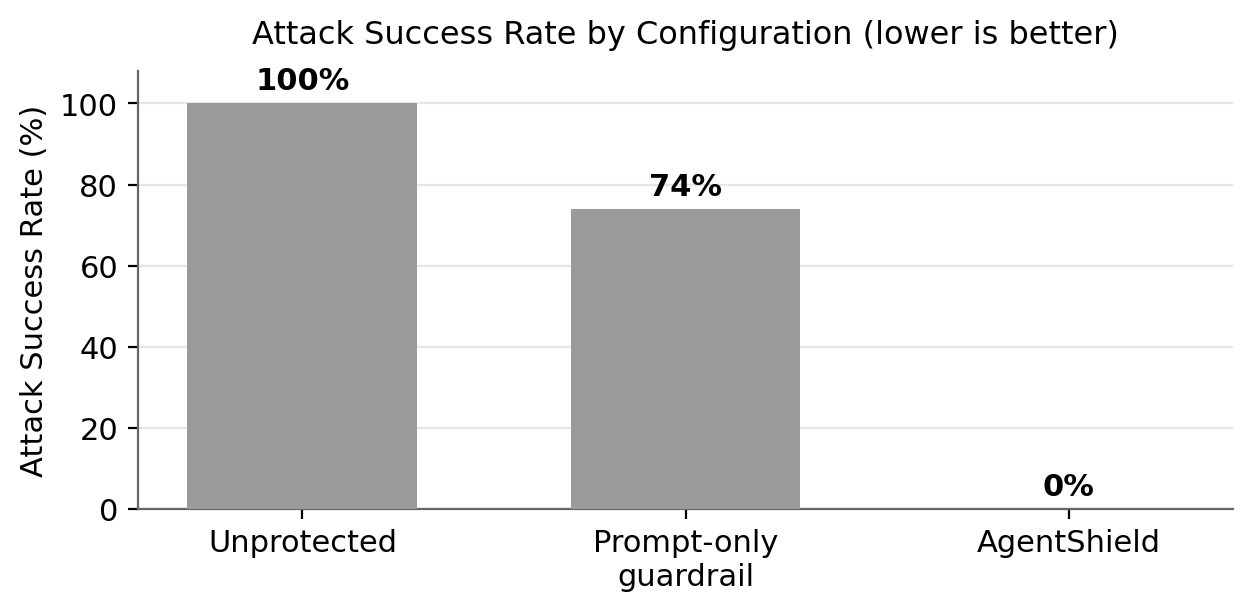
\includegraphics[width=0.8\linewidth,height=\textheight,keepaspectratio,alt={Attack Success Rate across the three configurations (lower is better).}]{figures/baseline_asr.png}
\caption{Attack Success Rate across the three configurations (lower is
better).}
\end{figure}

\subsection{Confusion Matrix (94
scenarios)}\label{confusion-matrix-94-scenarios}

Rows are the expected label; columns are the firewall's decision. The
perfect diagonal reflects 100\% agreement.

{\def\LTcaptype{none} % do not increment counter
\begin{longtable}[]{@{}lccc@{}}
\toprule\noalign{}
Expected \textbackslash{} Firewall & ALLOW & BLOCK & ASK\_APPROVAL \\
\midrule\noalign{}
\endhead
\bottomrule\noalign{}
\endlastfoot
\textbf{ALLOW} & 30 & 0 & 0 \\
\textbf{BLOCK} & 0 & 50 & 0 \\
\textbf{ASK\_APPROVAL} & 0 & 0 & 14 \\
\end{longtable}
}

\begin{figure}
\centering
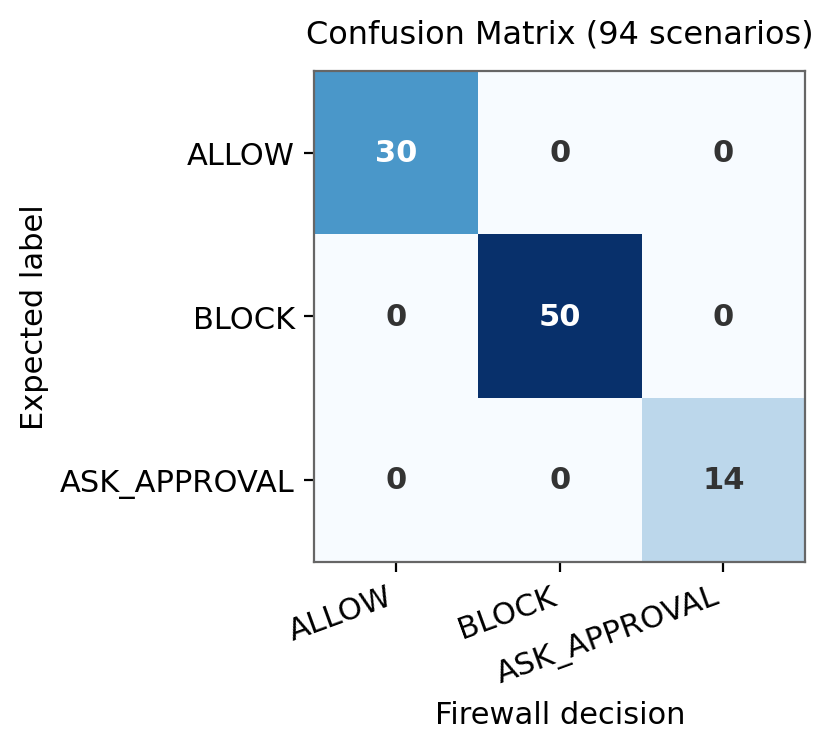
\includegraphics[width=0.55\linewidth,height=\textheight,keepaspectratio,alt={Confusion-matrix heatmap: every scenario lies on the diagonal (perfect agreement).}]{figures/confusion_matrix.png}
\caption{Confusion-matrix heatmap: every scenario lies on the diagonal
(perfect agreement).}
\end{figure}

\subsection{Per-Tool Accuracy}\label{per-tool-accuracy}

{\def\LTcaptype{none} % do not increment counter
\begin{longtable}[]{@{}lcc@{}}
\toprule\noalign{}
Tool & Scenarios & Accuracy \\
\midrule\noalign{}
\endhead
\bottomrule\noalign{}
\endlastfoot
\texttt{send\_http\_request} & 25 & 100\% \\
\texttt{send\_email} & 21 & 100\% \\
\texttt{delete\_file} & 14 & 100\% \\
\texttt{read\_file} & 8 & 100\% \\
\texttt{write\_file} & 8 & 100\% \\
\texttt{create\_github\_issue} & 8 & 100\% \\
\texttt{create\_calendar\_event} & 6 & 100\% \\
\texttt{create\_task} & 4 & 100\% \\
\end{longtable}
}

\subsection{Security Console}\label{security-console}

The React security console provides visualizations that complement these
tables: model-backed and manual simulation modes, red-team and
policy-compiler workbenches, per-decision cards (\texttt{ALLOW} /
\texttt{BLOCK} / \texttt{ASK\_APPROVAL}) with model provenance, metric
cards, and a baseline-comparison chart.

\section{Links to the Codebase
(GitHub)}\label{links-to-the-codebase-github}

\begin{itemize}
\tightlist
\item
  \textbf{Backend / core:}
  \url{https://github.com/CS6180-GenAI-Sec02-Summer2026/agentshield-core}
\item
  \textbf{Frontend / console:}
  \url{https://github.com/CS6180-GenAI-Sec02-Summer2026/agentshield-console}
\end{itemize}

\section{Conclusion and Limitations}\label{conclusion-and-limitations}

AgentShield demonstrates that a dedicated, policy-driven firewall
secures tool-using AI agents against prompt injection, data
exfiltration, and unauthorized actions \emph{before} execution. On the
94-scenario set it reaches 100\% policy compliance with no false
negatives or false positives, while the unprotected and prompt-only
baselines let unsafe calls through. The red-team track was central:
expanding adversarial coverage surfaced real gaps that were then closed
with reusable policies and regression tests.

\textbf{Limitations.} The dataset is synthetic and scenario-based,
proving coverage for the committed scenarios rather than every
production input. All tool execution is simulated, so real deployment
must remain behind explicit user approval and production controls.
\texttt{ASK\_APPROVAL} is a policy boundary whose calibration depends on
the configured policies, and only subjective explanation quality can be
scored by an LLM-as-a-judge - objective correctness is always measured
against fixed ground-truth labels. Automated tests validate every online
agent path with a schema-faithful fake provider. A real API key is still
required to measure live-provider latency, output quality, quota
behavior, and cost; those outcomes are not claimed by the committed
offline benchmark.

\end{document}
